%	LaTeX template for the Collaborative Research Center proposal (3rd funding period) Oxyflame.
%	WSA, RWTH Aachen, 2020, (contact person: Stefan Pielsticker)

%%%% PLEASE ADJUST:
%\WorkInstruction{ Enter the number of the project here. Replace only the text "Example project" Please make sure that the project name corresponds exactly to the name of the folder of your project.}
% Example: \renewcommand{\Project}{A1}

\renewcommand{\Project}{A1}
\renewcommand{\ChapterTitle}{Gasphase modelling}
\renewcommand{\ProjectTitle}{Original title from DFG proposal}

\newcommand*\positioncircle[1]{\raisebox{.5pt}{\textcircled{\raisebox{-.9pt} {#1}}}}


%%%% DON'T CHANGE ANYTHING FROM HERE UNTIL NEXT MARKER!
\chapter{\ChapterTitle}
%%%% DONT CHANGE ANYTHING UNTIL HERE!

%%%% PLEASE ADJUST:
\chapterauthor[1]{Anita Meraviglia}
\chapterauthor[1]{Pooria Farmand}
\chapterauthor[2]{Leon Loni Berkel}
\chapterauthor[3]{Stefan Pielsticker}
\chapterauthor[3]{Reinhold Kneer}
\chapterauthor[2]{Christian Hasse}
\chapterauthor[1]{Heinz Pitsch}

%%%% DON'T CHANGE ANYTHING FROM HERE UNTIL NEXT MARKER!
\begin{affils}
	%%%% DONT CHANGE ANYTHING UNTIL HERE!
	
	%%%% PLEASE ADJUST:
	\chapteraffil[1]{\RWTHITV}
	\chapteraffil[2]{\RWTHWSA}
	
%%%% DON'T CHANGE ANYTHING FROM HERE UNTIL NEXT MARKER!
\end{affils}
\begin{refsection}

\begin{abstract}
\label{sec:\Project _Abstract}
%%%% DONT CHANGE ANYTHING UNTIL HERE!

%%%% PLEASE ADJUST
%\WorkInstruction{Title: Keep it short and make sure that it fits well with the part title and the other project titles within that part. Therefore see the planned chapter outline in section~\ref{ex: chap Outline}.}

%\WorkInstruction{Author List: If you use data from FP1/FP2 members, please list them here as well.}

%\WorkInstruction{Affiliations: Please use the commands already prepared (\textbackslash RWTHWSA, \textbackslash RWTHAIA, \textbackslash RWTHITV, \textbackslash RUBLEAT, \textbackslash RUBLTC, \textbackslash RUBThermo, \textbackslash RUBTC, \textbackslash RUBACII, \textbackslash TUDSTFS,\textbackslash TUDRSM, \textbackslash TUDEST. For changes or other affiliations text us.}

% Abstract
Oxy-fuel combustion provides several significant advantages, such as a high \ce{CO2} content and reduced \ce{NO_x} emissions. The aim is to provide skeletal chemical kinetic models that can be coupled with a detailed solid particle model to model coal and biomass solid fuel combustion under oxy-fuel conditions. Extensively validated detailed chemical kinetic models are applied and reduced in a multi-step reduction approach to develop skeletal kinetic models for the gas phase kinetic of coal and biomass combustion. The obtained chemical kinetic models are validated according to their reduction goal for the application in simulations under fuel-lean, high temperature, and atmospheric pressure conditions. The \ce{NO_x} sub-model is developed to be coupled with a detailed solid particle model for nitrogen release. Considering all volatile species requires an accurate prediction of main \ce{NO_x} formation pathways as well as the \ce{C5H5N}-chemistry.
\\
The validation results of the developed kinetic models show an overall good agreement with the respective experimentally data for all aspects of the respective developed kinetic model.
\end{abstract}



\newpage
\section{Introduction} 
Chemical kinetic models are essential when dealing with combustion phenomena as they provide crucial information regarding reaction rates, species transport, and temperature effects. In this Oxyflame project, numerical simulations are performed to analyse the partially premixed flame resulting from the combustion of solid coal and biomass particles. Like in Cha.~\linkproject{B3}, where solid particle DNS are performed to analyse the combustion and ignition behaviour as well as the main \ce{NO_x} formation pathways, these numerical simulations are conducted predominantly under high-temperature air and oxy-fuel conditions at atmospheric pressure. Therefore, with this application in mind, it is necessary to develop a chemical kinetic model to describe the underlying chemistry of the released volatile species in the surrounding gas phase of the solid particle. The latter is determined by employing the solid particle model for coal and biomass devolatilisation from Cha.~\linkproject{A8}, which leads to the definition of a complex mixture ranging from light hydrocarbons and oxygenated species up to heavy lignin tars (\ce{C24H28O4}) and aromatic compounds. Considering the \ce{NO_x} sub-model from Cha.~\linkproject{A8}, various nitrogen-containing species are released to the gas phase, and the introduction in the kinetic model of the relevant chemistry describing their evolution in the combustion system is essential for accounting for the main \ce{NO_x} formation pathways.
\\
Detailed chemical kinetic models aim to describe the combustion process as accurately as possible. However, this might require hundreds or even thousands of species and reactions. Since the computational cost of complex simulations typically increases as the number of species in the employed kinetic model grows, developing skeletal kinetic models with a reduced number of species and reactions while preserving high accuracy is of key importance for performing the simulation of interest that would be otherwise computationally prohibitive.
\\
Present kinetic models for coal and biomass combustion in the literature are either not adapted to the solid particle model from Cha.~\linkproject{A8}, do not contain large aromatic species, or are not validated for the application under oxy-fuel conditions~\cite{Shamooni2021, Goyal2017, Lovas2013}. In addition, most of the kinetic models for \ce{NO_x} formation in the literature do not contain all volatile species released from the solid nitrogen particle model like the model from Glarborg et al.~\cite{Glarborg2018} or are not well documented~\cite{Shamooni2021}. 
\\
The development of chemical kinetic models for the gas phase kinetic coupled with the solid particle model from Cha.~\linkproject{A8} is presented in this chapter. The first part delves into the development process of skeletal coal and biomass combustion models and a modular \ce{NO_x} model. The second part focuses on validating these chemical kinetic models.



\newpage
\section{Chemical kinetic model development}
The development of chemical kinetic models for coal and biomass combustion is presented in this section. A reduced version of the model from Cai et al.~\cite{Cai2020} is developed for coal combustion. According to this model, the development of recent kinetic models for coal and biomass combustion is discussed. These recent developed models are developed to be adapted to the solid particle model from Cha.~\linkproject{A8}. A modular \ce{NO_x} model is developed based on the solid particle model, which is presented at the end of this section.


\subsection{Development of skeletal coal and biomass models}
A skeletal kinetic model for coal combustion is developed based on the model from Cai et al.~\cite{Cai2020}. The model from Cai et al.~\cite{Cai2020} is based on a kinetic model from Blanquart et al.~\cite{Blanquart2009} to describe the oxidation of a set of \ce{C0} to \ce{C4} hydrocarbon fuels including \ce{CH4}. This base-chemistry is extended to include the formation of polycyclic aromatic hydrocarbon according to the study from Narayanaswamy et al.~\cite{Narayanaswamy2010} and is refined by incorporating the hydrogen mechanism from Burke et al.~\cite{Burke2012}. Further details about the development process can be found in Ref.~\cite{Cai2020}. The model from Cai et al.~\cite{Cai2020} is extensively validated for the combustion of fuels in air~\cite{Cai2019} and for the oxy-methane combustion~\cite{Cai2020}. A skeletal kinetic model based on the model from Cai et al.~\cite{Cai2020} is developed and validated for the ignition delay time of \ce{CH4} under air and oxy-fuel conditions. This reduced kinetic model is named ITV-2020, containing 68 species and 906 reactions.
\\
In comparison to the ITV-2020 model, recently developed skeletal kinetic models for coal and biomass combustion are tailored to the solid particle model from Cha.~\linkproject{A8}. These models are developed to predict the ignition delay time and the respective fuel chemistry to be employed to simulate the respective gas-phase kinetics under high-temperature and atmospheric pressure conditions. The development of these recent skeletal kinetic models for coal and biomass combustion involves a multi-step reduction strategy using detailed chemical kinetic models. The reduction stage aims to develop chemical kinetic models with a limited number of species while accurately describing the evolution of volatile species under the specific conditions of interest. A schematic of the whole reduction strategy is summarized in Fig.~\ref{fig:B1bKineticModelDevelopmentStructure}.
% Mechanism development strategy
\begin{figure}[h]
  \centering
  \subfloat{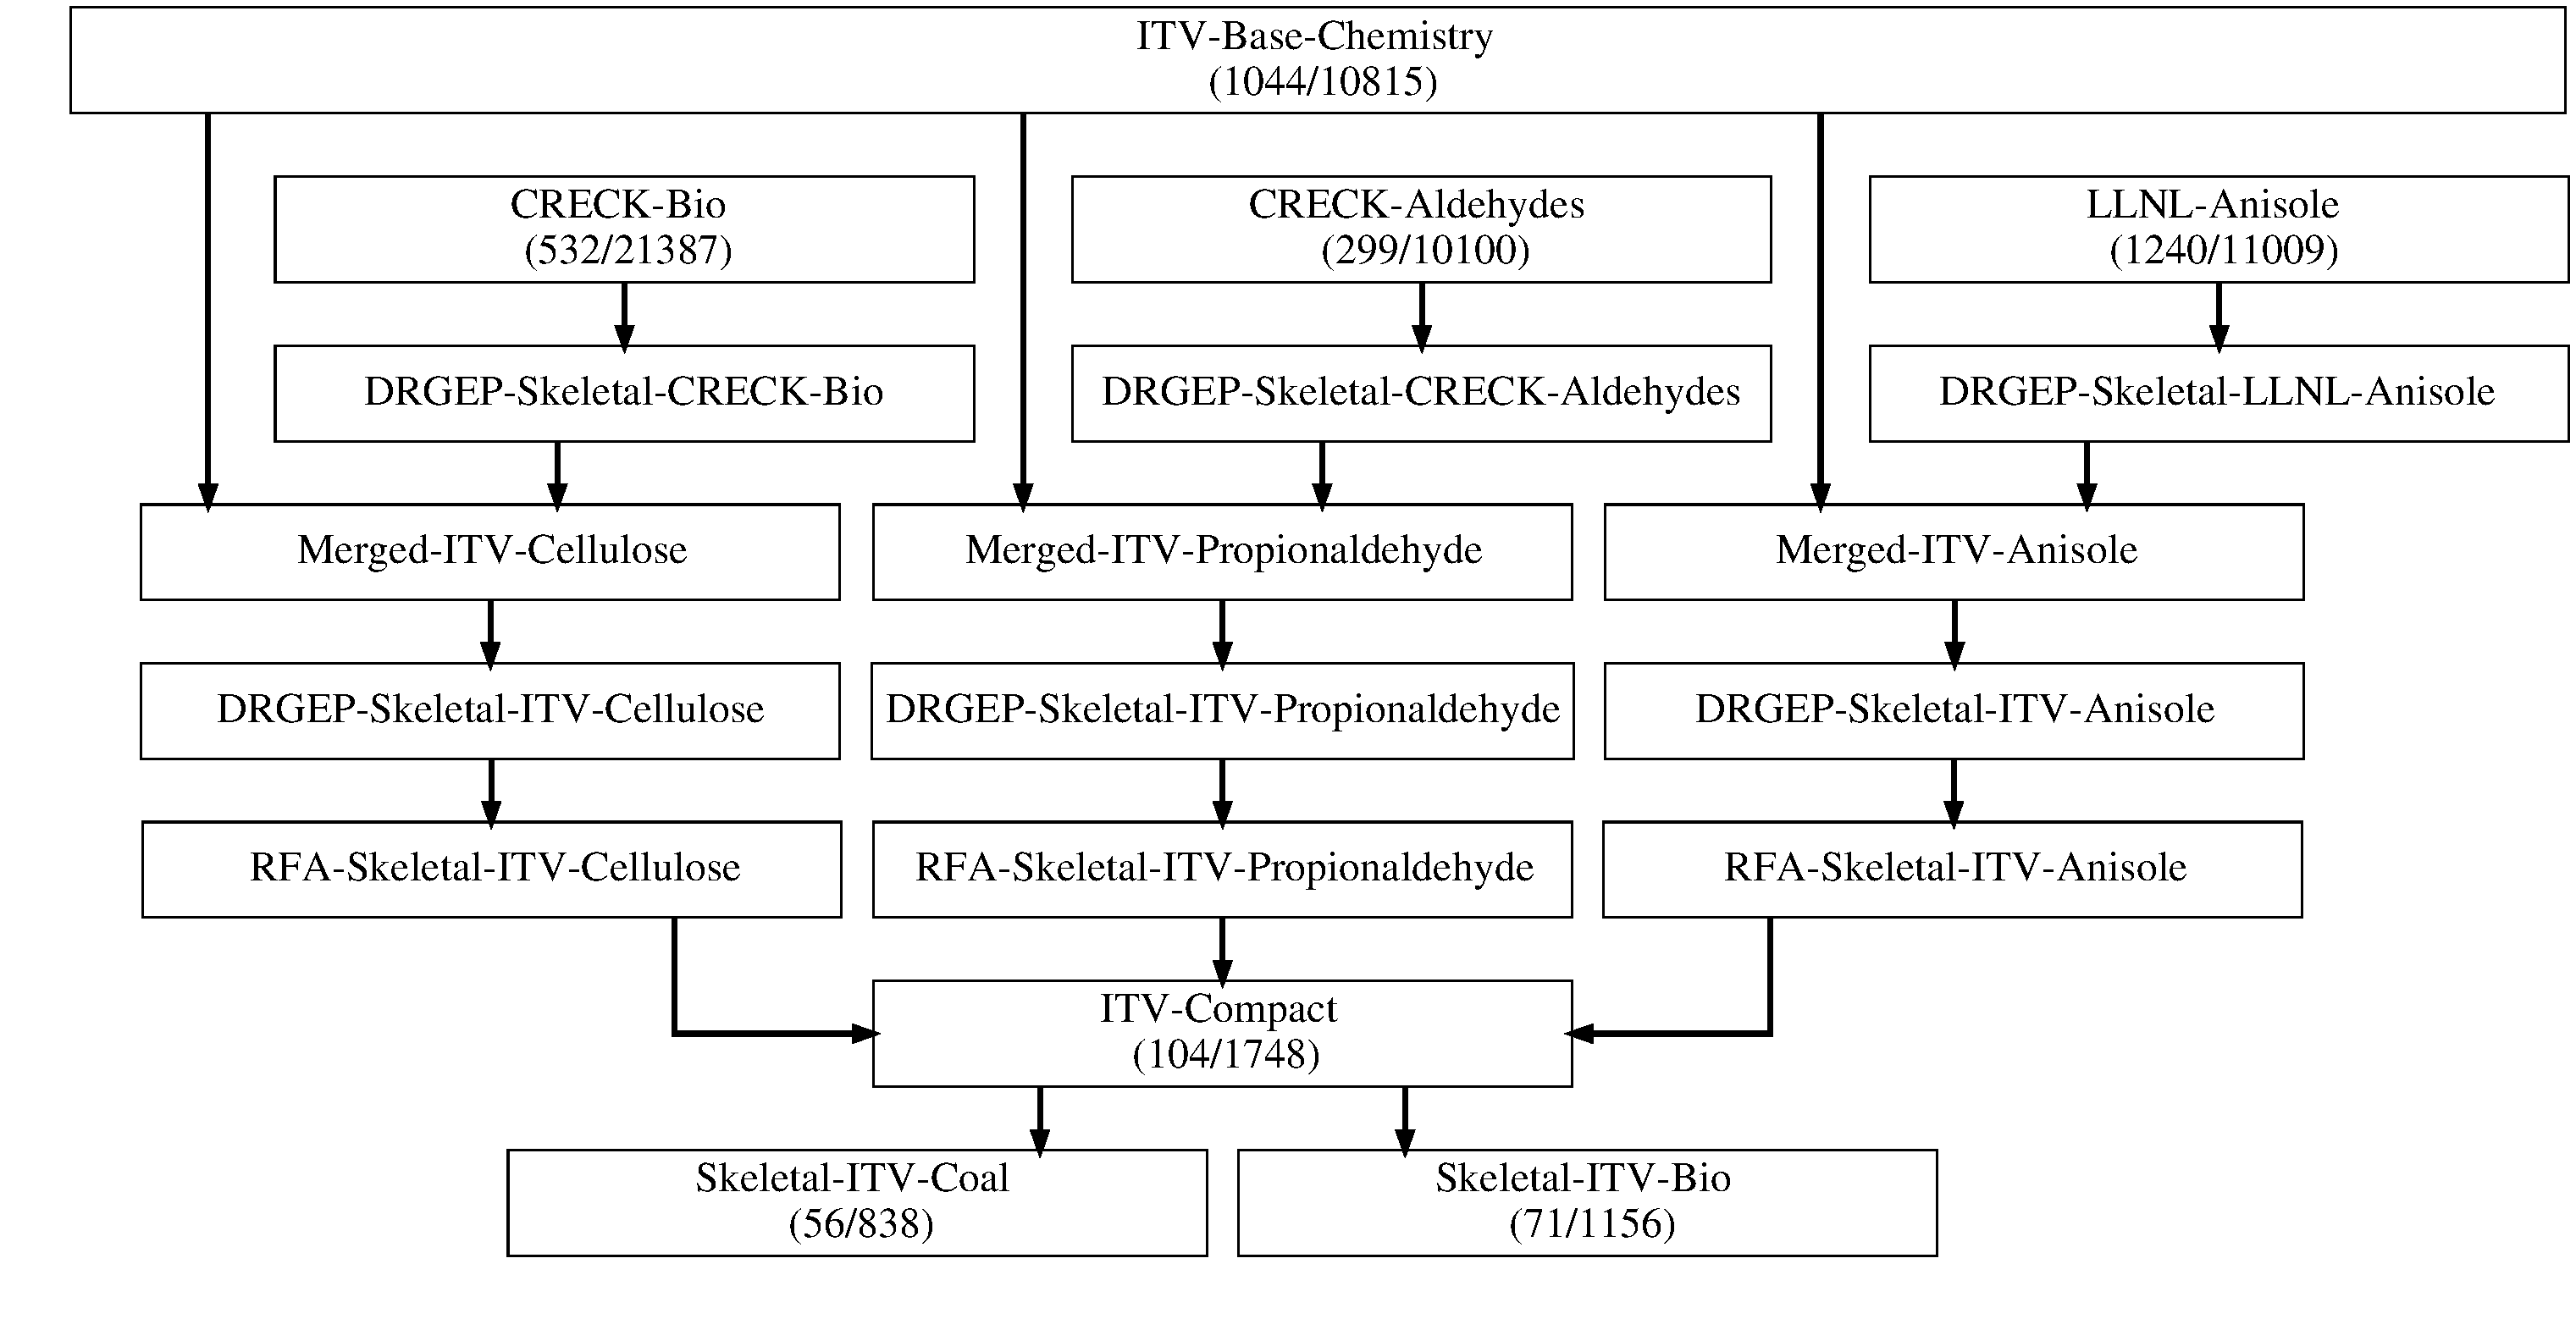
\includegraphics[width=1.0\textwidth]{\ThisPath Figures/B1b_FlowChartMechanismDevelopment.pdf}}
  \caption{Flow chart for developing the skeletal gas phase mechanisms for coal (Skeletal-ITV-Coal) and biomass (Skeletal-ITV-Bio) combustion. The initial mechanisms are the ITV-Base-Chemistry from Langer et al.~\cite{Langer2023}, the CRECK-Bio~\cite{Debiagi2016}, the CRECK-Aldehydes~\cite{Pelucchi2015}, and the LLNL-Anisole model~\cite{Wagnon2018}.}
  \label{fig:B1bKineticModelDevelopmentStructure}
\end{figure}
\\
According to the devolatisation model from Cha.~\linkproject{A8}, coal and biomass particles release a complex mixture of volatile species to the gas phase. One of the dominant volatile species released during coal and lignin combustion is anisole, while levoglucosan is the dominant volatile species released from cellulose combustion. To describe the ignition delay time of coal and biomass combustion, the chemistry of anisole and propionaldehyde is considered, the most dominant species released at particle temperatures where biomass ignites is observed, based on model simulations with the solid particle model from Cha.~\linkproject{A8}. However, these species are not included in the detailed model from Langer et al.~\cite{Langer2023}. To integrate these missing species chemistry in the model from Langer et al.~\cite{Langer2023}, extensively validated detailed chemical kinetic models are used to describe the respective chemistry of interest over a broad range of conditions. The missing anisole chemistry has been adopted from the model of Wagnon et al.~\cite{Wagnon2018}, cellulose volatile species from Debiagi et al.~\cite{Debiagi2016}, and the propionaldehyde chemistry from Pelucchi et al.~\cite{Pelucchi2015}.
\\
The extensively validated model from Langer et al.~\cite{Langer2023} has been systematically extrapolated from recently published chemical kinetic models and combined with these recently published detailed chemical kinetic models~\cite{Wagnon2018, Debiagi2016, Pelucchi2015}, describing the missing volatile species chemistry. The integration of the chemistry, describing the gas phase kinetics of these volatile species, into the model from Langer et al.~\cite{Langer2023} has been achieved using a systematic approach. In order to extrapolate only the relevant chemistry for the species, the Direct Relation Graph with Error Propagation (DRGEP) method~\cite{PepiotDesjardins2008a} has been applied to these detailed models. The obtained reduced chemical kinetic models are merged into the detailed model from Langer et al.~\cite{Langer2023} based on InChIs and SMILES for each species. Only the species and reactions, as well as the species thermodynamic and transport data, are extracted and added to the chemical kinetic model from Langer et al.~\cite{Langer2023}, which are not included.
\\
The so obtained kinetic models are referred to as "Merged-ITV-Cellulose", "Merged-ITV-Propionaldehyde", and "Merged-ITV-Anisole", as shown in Fig.~\ref{fig:B1bKineticModelDevelopmentStructure}. The obtained models undergo a multi-step reduction strategy involving the DRGEP method~\cite{PepiotDesjardins2008a} and Reaction Flux Analysis. A reaction flux analysis allows a flexible and targeted extraction of major formation and consumption pathways of the species of interest from the mechanism, while the DRGEP method~\cite{PepiotDesjardins2008a} is a more conservative reduction method. The extraction with the reaction flux analysis is performed based on the respective validation cases to consider the range of validity and application. The validation database presented in Ref.~\cite{Langer2023} is expanded in this work by integrating additional speciation data representative of anisole oxidation~\cite{Chen2022}, cellulose pyrolisis~\cite{Norinaga2013}, and shock tube ignition-delay time measurements of anisole and propionaldehyde~\cite{Pelucchi2015, AkihKumgeh2011}.
\\
Skeletal kinetic models from each reduction step are named employing the prefixes "DRGEP-Skeletal" and "RFA-Skeletal" in Fig.~\ref{fig:B1bKineticModelDevelopmentStructure}, followed by the name of the corresponding detailed chemical kinetic model. The reduction process allows the retention of only the relevant chemistry for the species of interest. This allows the merging process of the skeletal models to be more straightforward, leading to a compact chemical kinetic model (ITV-Compact) able to accurately describe the evolution of the volatile species released from coal and biomass.
\\
The final reduction step contains a DRGEP step and an additional reduction step using the reaction flux analysis to obtain skeletal chemical kinetic models for coal and biomass combustion. These skeletal kinetic models describe the gas phase kinetics of volatile species released from coal (Skeletal-ITV-Coal) and biomass (Skeletal-ITV-Bio). The applicability of both models can be emphasized by the fact that the Skeletal-ITV-Coal and the Skeletal-ITV-Bio mechanisms contain several volatile species released from the solid particle model from Cha.~\linkproject{A8}.


\subsection{Development of a \ce{NOx} chemical kinetic sub-model}
To describe the formation of \ce{NO_x} from nitrogen-containing volatile species released from the solid particle model from Cha.~\linkproject{A8}, a chemical kinetic gas-phase model for \ce{NO_x} formation is newly developed. This newly developed chemical kinetic model uses an ITV-\ce{NO_x} model, a reduced version of the well-documented Glarborg model~\cite{Glarborg2018}, crafted through ab-initio and experimental studies, as base chemistry. As a result of Girhe et al.~\cite{Girhe2024}, the ammonia chemistry from the KAUST model is integrated into the ITV-\ce{NO_x} model to improve the predictions of the ammonia chemistry. The pyridine chemistry to model tar-N is adopted from the CRECK-\ce{NO_x} model~\cite{Shamooni2021} and integrated into the base-chemistry model.
\\
A reaction rate modification is applied since this merged ITV-\ce{NO_x} model over-predicts the \ce{NO} formation over a broad range of experimental conditions. A rate parameter adoption from the CRECK-\ce{NO_x} model~\cite{Shamooni2021} (reaction: $\ce{NCO}+\ce{O} \Leftrightarrow \ce{NO}+\ce{CO}$) and a minor tuning of the frequency parameter (reaction: $\ce{NCO}+\ce{NO} \Leftrightarrow \ce{N2O}+\ce{CO}$) result in an accurate prediction of the \ce{NO} chemistry (Complete-ITV-\ce{NO_x}).
\\
Next to the rate modifications, the nitrogen chemistry in the Complete-ITV-\ce{NO_x} model is extracted using the reaction flux analysis to obtain a more compact model size. Considering the validation cases from Alzueta et al.~\cite{Alzueta2002} and Wu et al.~\cite{Wu2019, Wu2022}, a modular Skeletal-ITV-\ce{NO_x} kinetic model is obtained, which covers a broad spectrum of fuel-air ratios, temperatures, and initial conditions with 36 species and 595 reactions.




\newpage
\section{Validation of kinetic models}
The skeletal chemical kinetic models are developed to predict the ignition delay time and respective fuel chemistry based on detailed chemical kinetic models. However, due to the reduction of detailed chemical kinetic models, the prediction accuracy of the chemistry of several species is affected. Consequently, a comprehensive validation is required to cover all relevant fuels and target species and include ignition delay times and speciation data in a broad range of temperatures at atmospheric pressure. Numerical simulations for the validation are performed using appropriate models in the FlameMaster code~\cite{Pitsch1990}.


\subsection{Skeletal kinetic models for coal combustion}
This subsection provides a validation of the ITV-2023 kinetic model for coal combustion and the ITV-2020 model, covering all aspects of the respective development goals.
\\
The ITV-2020 coal model is developed to predict the ignition delay time of methane under oxy-fuel conditions. Figure~\ref{fig:B1bIDTLimingCaiCoalMechanism} shows model predictions of the ITV-2020 model in comparison with experimental shock-tube measurements from Koroglu et al.~\cite{Koroglu2016}. Koroglu et al.~\cite{Koroglu2016} measures the ignition delay time for \ce{CH4}/\ce{O2}/\ce{CO2} mixtures in bath gas of \ce{Ar} for different pressures and equivalence ratios. As shown in Fig.~\ref{fig:B1bIDTLimingCaiCoalMechanism}, the ITV-2020 model satisfactorily predicts the ignition delay times for all conditions and temperature ranges.
% Ignition delay time validation - Koroglu
\begin{figure}[h]
  \centering
  \subfloat{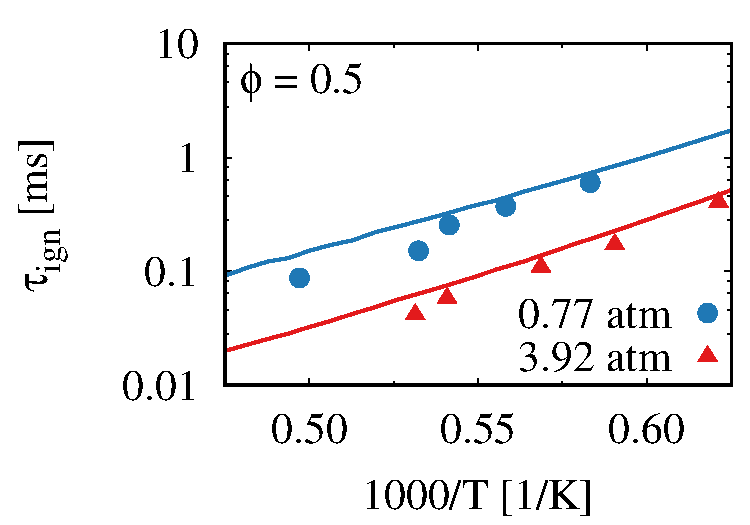
\includegraphics[width=0.32\textwidth]{\ThisPath Figures/B1b_LCai_IDT_CH4_Koroglu_Lean.pdf}}
  \hfill
  \subfloat{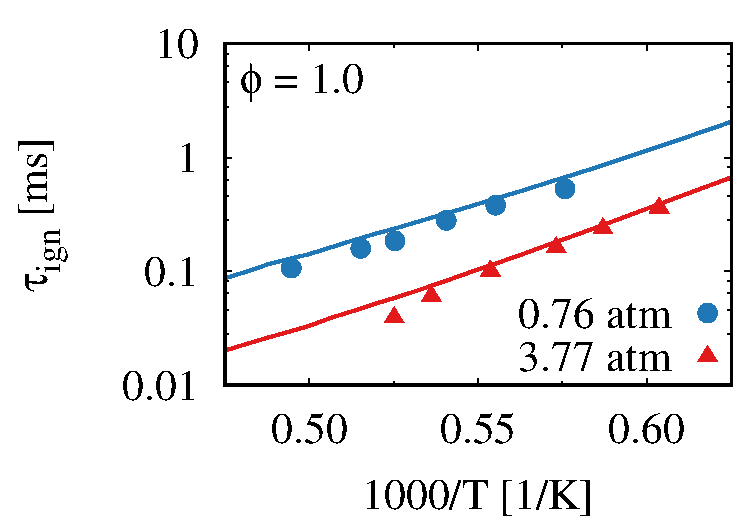
\includegraphics[width=0.32\textwidth]{\ThisPath Figures/B1b_LCai_IDT_CH4_Koroglu_Stoi.pdf}}
  \hfill
  \subfloat{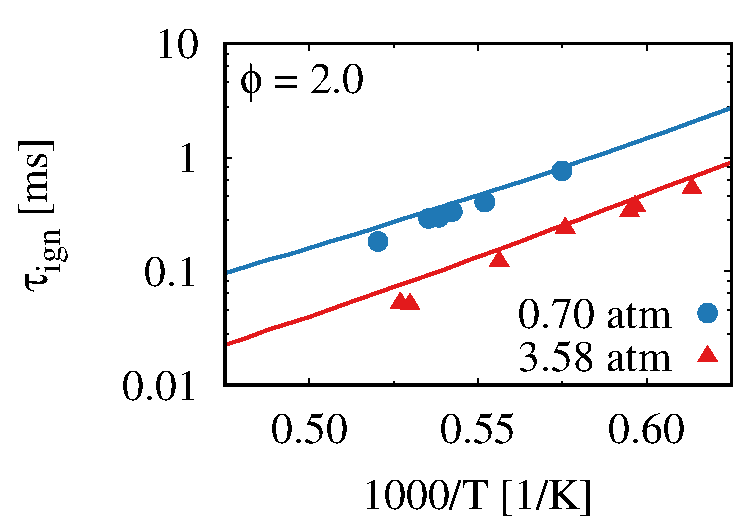
\includegraphics[width=0.32\textwidth]{\ThisPath Figures/B1b_LCai_IDT_CH4_Koroglu_Rich.pdf}}
  \caption{Comparison of experimental measured ignition delay times of \ce{CH4}/\ce{O2}/\ce{CO2}/\ce{Ar} mixtures from Koroglu et al.~\cite{Koroglu2016} with model predictions of the ITV-2020 model.}
  \label{fig:B1bIDTLimingCaiCoalMechanism}
\end{figure}
% Ignition delay time validation
\begin{figure}[t]
  \centering
  \subfloat{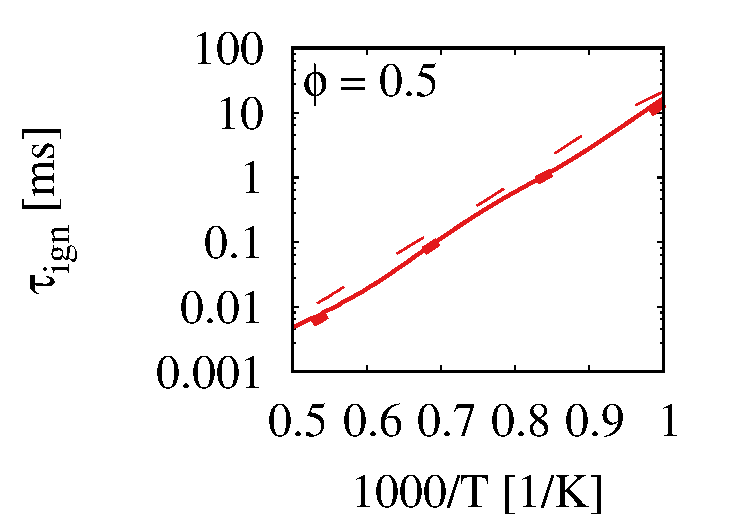
\includegraphics[width=0.32\textwidth]{\ThisPath Figures/B1b_Coal_IDT_Lean_1atm.pdf}}
  \hfill
  \subfloat{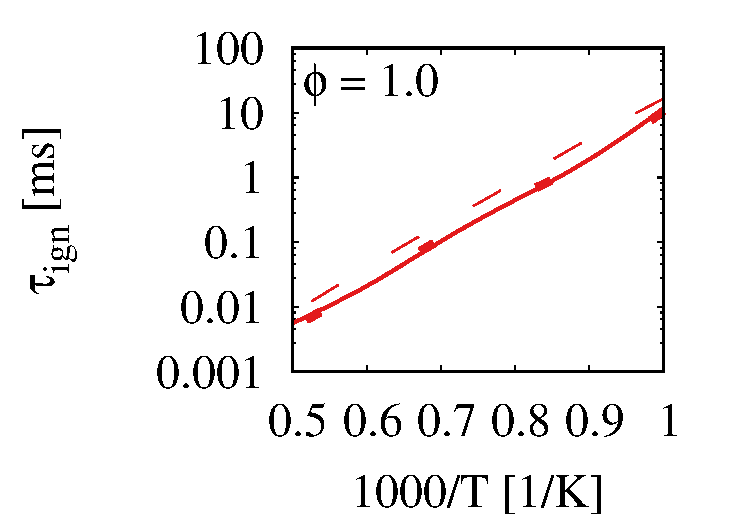
\includegraphics[width=0.32\textwidth]{\ThisPath Figures/B1b_Coal_IDT_Stoichiometric_1atm.pdf}}
  \hfill
  \subfloat{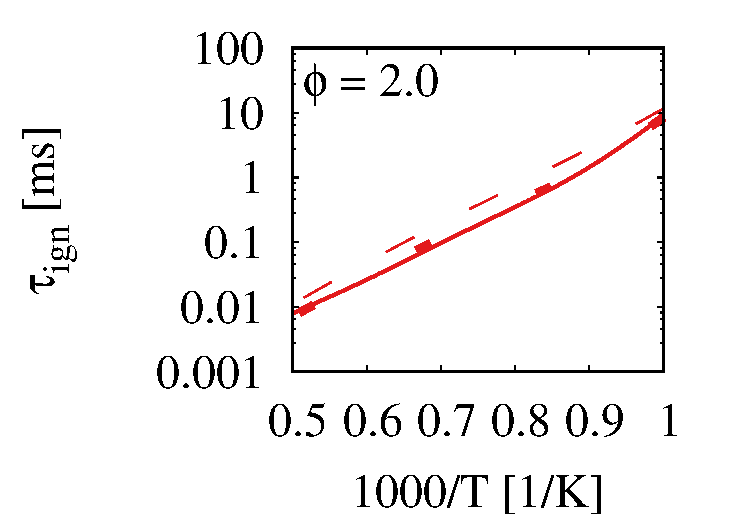
\includegraphics[width=0.32\textwidth]{\ThisPath Figures/B1b_Coal_IDT_Rich_1atm.pdf}}
  \caption{Model comparison for the ignition delay times of anisole/air mixtures at atmospheric pressure for the Skeletal-ITV-Coal model (solid lines), the Merged-ITV-Anisole model (dotted lines), and the LLNL-Anisole model~\cite{Wagnon2018} (dashed lines).}
  \label{fig:B1bIDTAnisoleCoalMechanism}
\end{figure}
\\
The ITV-2023 coal skeletal model is validated by considering the oxidation of anisole at atmospheric pressure over a broad range of temperatures. Quantities predicted by the skeletal model are compared against the ones of the corresponding detailed model to assess the effect induced by the reduction phase. Additionally, to assess the influence of differing base chemistry, the performance of the ITV-based detailed chemical kinetic model is evaluated against both the reference models and, where possible, experimental data. The detailed chemical kinetic model from Wagnon et al.~\cite{Wagnon2018} and the Merged-ITV-Anisole mechanism serve as a reference for the skeletal chemical kinetic model in both cases.
\\
Figure~\ref{fig:B1bIDTAnisoleCoalMechanism} compares the model prediction for the ignition delay time of anisole/air mixtures for the Skeletal-ITV-Coal, the Merged-ITV-Anisole, and the LLNL-Anisole model~\cite{Wagnon2018} models. Model predictions for the ignition delay times of the Skeletal-ITV-Coal and the Merged-ITV-Anisole model are similar, indicating a low error in the mechanism reduction process. The difference in the prediction of the ignition delay time compared to the LLNL-Anisole model~\cite{Wagnon2018} is based on the different base chemistry in the models.
% Ansiole oxidation chemistry - oxy conditions
\begin{figure}[b]
  \centering
  \subfloat{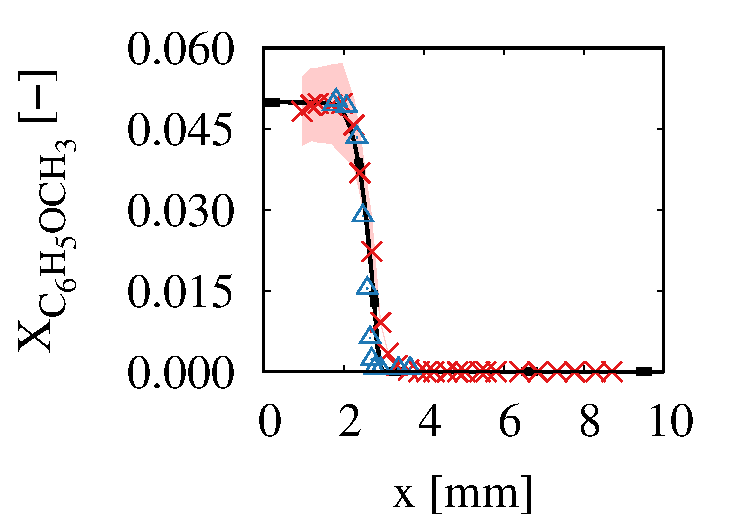
\includegraphics[width=0.32\textwidth]{\ThisPath Figures/B1b_Coal_Figure_6a.pdf}}
  \hfill
  \subfloat{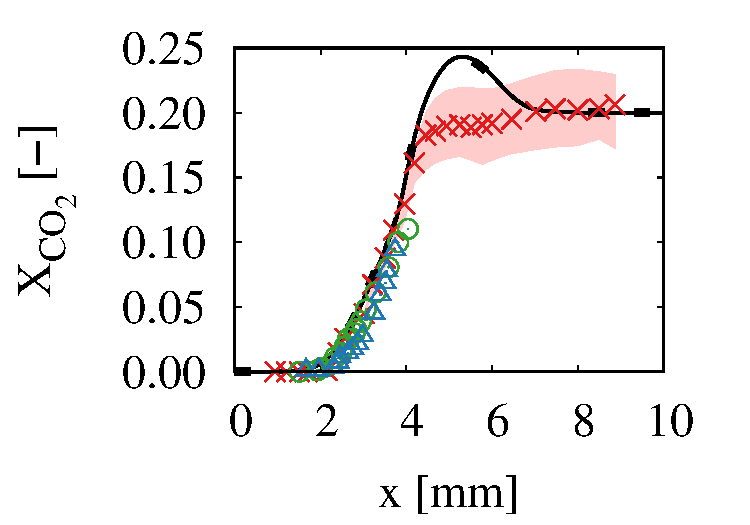
\includegraphics[width=0.32\textwidth]{\ThisPath Figures/B1b_Coal_Figure_6f.pdf}}
  \hfill
  \subfloat{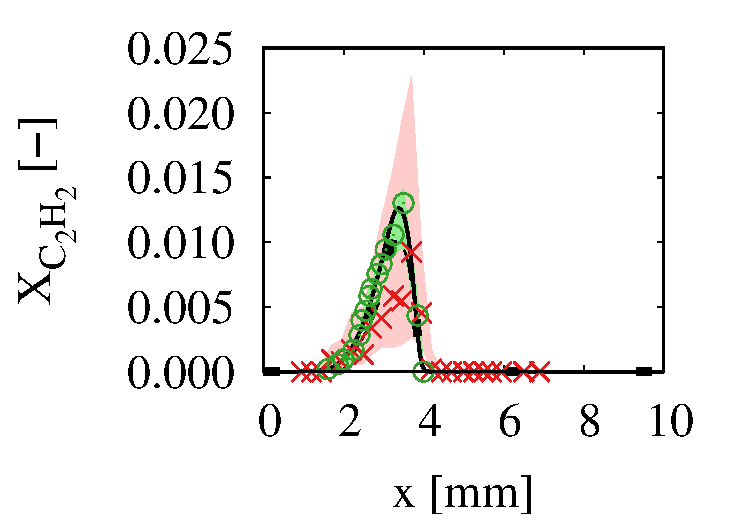
\includegraphics[width=0.32\textwidth]{\ThisPath Figures/B1b_Coal_Figure_8b.pdf}}
  \caption{Comparison of experimentally measured mole fractions in the \ce{CO2}O-Flame for anisole oxidation from Chen et al.~\cite{Chen2022} (ToF-MBMS: red crosses; GC-MS with a Rt-Q-Bond column: green circles; GC-MS with a DB-Petro column: blue triangles) with model predictions of the Skeletal-ITV-Coal (solid lines), the Merged-ITV-Anisole (dotted lines), and the LLNL-Anisole model~\cite{Wagnon2018} (dashed lines). Shaded areas with different colours indicate the measurement uncertainty of the respective techniques. x refers to the distance from the fuel inlet at 0 mm to the oxidizer inlet at 10 mm.}
  \label{fig:B1bAnisoleOxidationCoalMechanismCO2O}
\end{figure}
\\
The validation of the anisole oxidation chemistry for the Skeletal-ITV-Coal model is given based on the experimental study from Chen et al.~\cite{Chen2022}. An examined flame configuration from Chen et al.~\cite{Chen2022} contains carbon dioxide as diluent on the oxidizer side (\ce{CO2}O-Flame) to represent oxy-fuel conditions as discussed in Cha.~\linkproject{B1}. Figure~\ref{fig:B1bAnisoleOxidationCoalMechanismCO2O} compares the Skeletal-ITV-Coal model predictions with the respective detailed kinetic model predictions in the \ce{CO2}O-Flame. Anisole and \ce{CO2} model predictions of the Skeletal-ITV-Coal model show no discrepancies to the detailed LLNL-Anisole~\cite{Wagnon2018} and the Merged-ITV-Anisole. Model predictions of the Skeletal-ITV-Coal model the intermediate hydrocarbon species \ce{C2H2} captures the GC-MS measured mole fraction peak, while the Merged-ITV-Coal and the LLNL-Anisole model~\cite{Wagnon2018} are both under-predicting the mole fraction peak.


\subsection{Skeletal kinetic model for biomass combustion}
Applying the newly developed skeletal kinetic model for biomass combustion requires a detailed validation of the ignition delay time and the chemistry of levoglucosan and anisole in a predefined range of validity. The Skeletal-ITV-Bio model is built on the detailed chemical kinetic models of CRECK-Aldehydes~\cite{Pelucchi2015}, CRECK-Bio~\cite{Debiagi2016}, LLNL-Anisole~\cite{Wagnon2018}, and the updated ITV-Base-Chemistry~\cite{Langer2023}. These detailed chemical kinetic models are validated against data from several experimental species over various conditions. The newly developed Skeletal-ITV-Bio kinetic model will be validated for the ignition delay time of propionaldehyde, secondary pyrolysis of cellulose volatile species, and for the anisole oxidation chemistry against experimental data~\cite{Pelucchi2015, AkihKumgeh2011, Chen2022}.
% Ignition delay time validation
\begin{figure}[h]
  \centering
  \subfloat{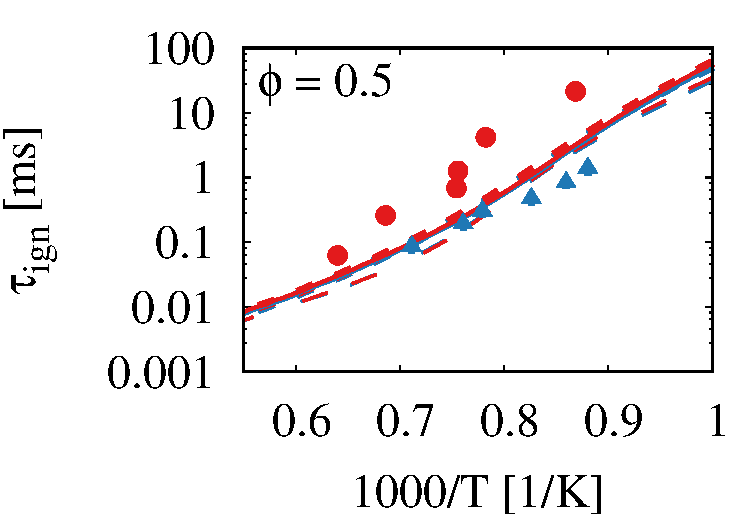
\includegraphics[width=0.32\textwidth]{\ThisPath Figures/B1b_Bio_IDT_Propanal_Lean.pdf}}
  \hfill
  \subfloat{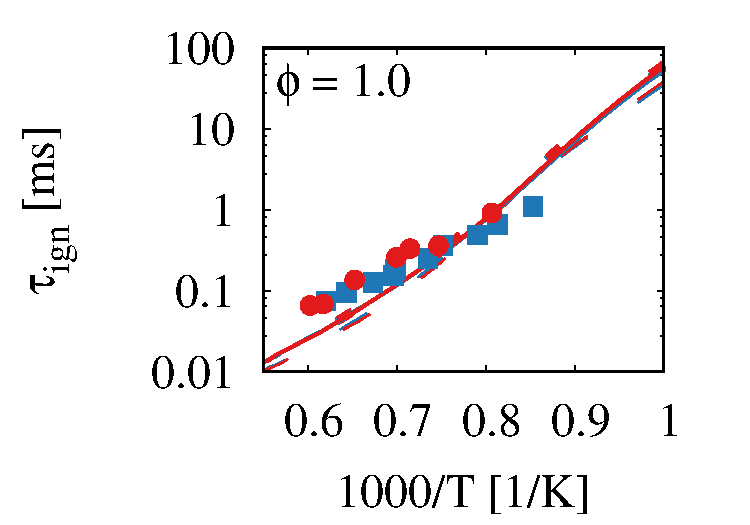
\includegraphics[width=0.32\textwidth]{\ThisPath Figures/B1b_Bio_IDT_Propanal_Stoichiometric.pdf}}
  \hfill
  \subfloat{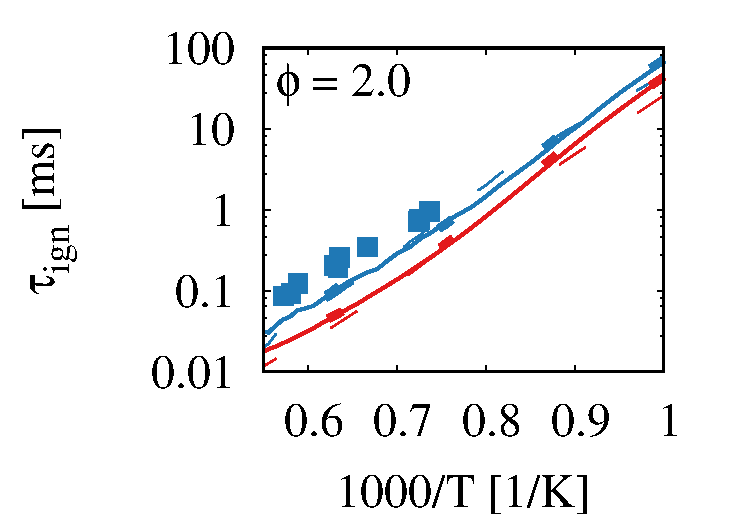
\includegraphics[width=0.32\textwidth]{\ThisPath Figures/B1b_Bio_IDT_Propanal_Rich.pdf}}
  \caption{Comparison of the propionaldehyde ignition delay time for experimental shock-tube measurements from Pelucchi et al.~\cite{Pelucchi2015} (blue squares) and from Akih-Kumgeh and Bergthorson~\cite{AkihKumgeh2011} (black circles) with model predictions of the Skeletal-ITV-Bio model (solid lines), the Merged-ITV-Propionaldehyde model (dotted lines), and the CRECK-Aldehydes model~\cite{Pelucchi2015} (dashed lines).}
  \label{fig:B1bIDTPropionaldehydeBioMechanism}
\end{figure}
% Cellulose pyrolysis validation
\begin{figure}[t]
  \centering
  \subfloat{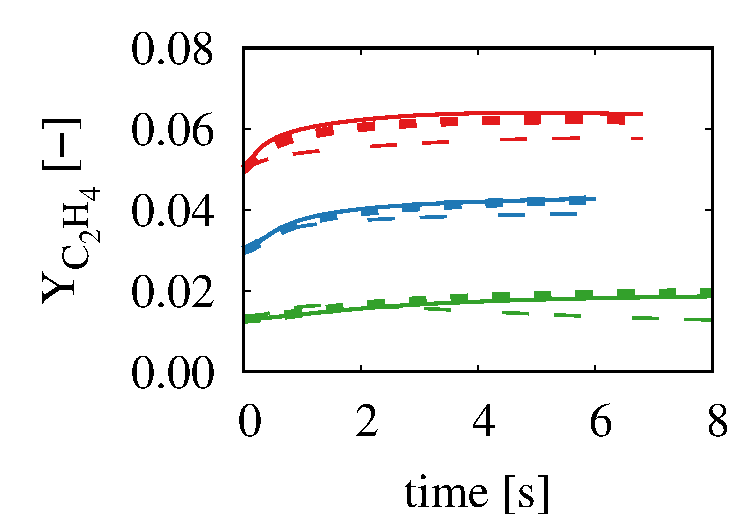
\includegraphics[width=0.32\textwidth]{\ThisPath Figures/B1b_Bio_CellulosePyrolysis_C2H4.pdf}}
  \hfill
  \subfloat{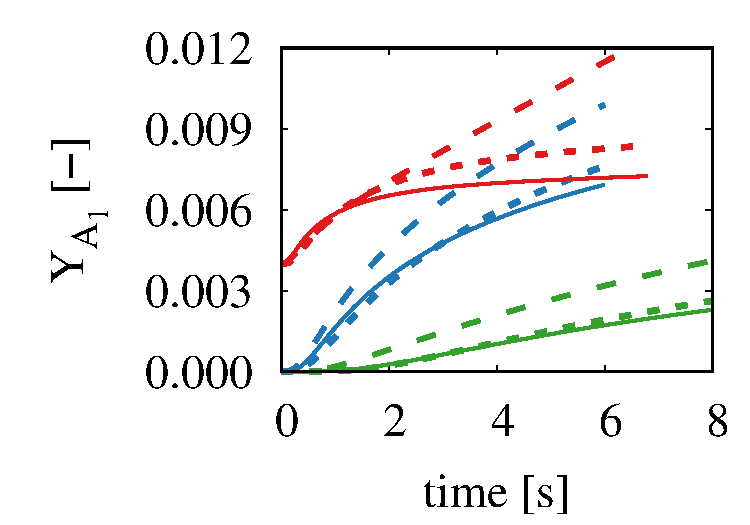
\includegraphics[width=0.32\textwidth]{\ThisPath Figures/B1b_Bio_CellulosePyrolysis_C6H6.pdf}}
  \hfill
  \subfloat{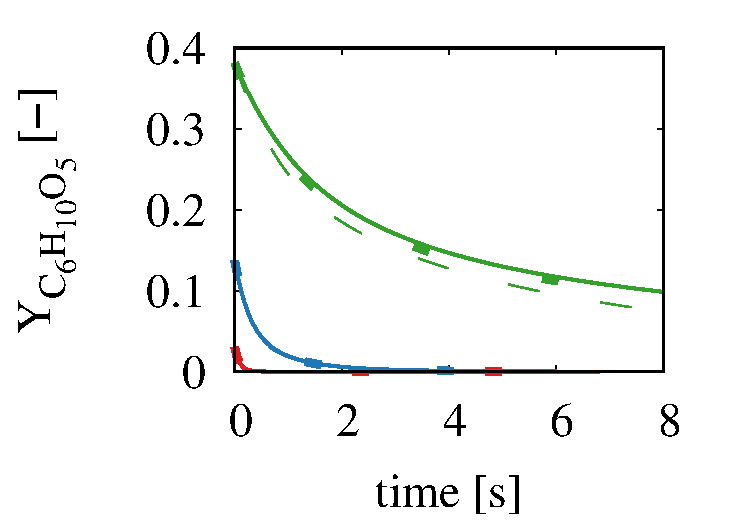
\includegraphics[width=0.32\textwidth]{\ThisPath Figures/B1b_Bio_CellulosePyrolysis_C6H10O5.pdf}}
  \caption{Model comparison for the secondary pyrolysis of cellulose volatile species at \SI{700}{\celsius} (green), \SI{750}{\celsius} (blue), and \SI{800}{\celsius} (red) for the Skeletal-ITV-Bio (solid lines), the Merged-ITV-Cellulose (dotted lines), and the CRECK-Bio model~\cite{Debiagi2016}.}
  \label{fig:B1bCellulosePyrolysisBioMechanism}
\end{figure}
\\
The ignition delay time for propionaldehyde is validated for three different fuel-air-equivalence ratios over a broad range of temperatures with experimental shock-tube measurements from Pelucchi et al.~\cite{Pelucchi2015} and Akih-Kumgeh and Bergthorson~\cite{AkihKumgeh2011}. Figure~\ref{fig:B1bIDTPropionaldehydeBioMechanism} compares the model predictions of the Skeletal-ITV-Bio model with the model predictions of the Merged-ITV-Propionaldehyde and the CRECK-Aldehydes model~\cite{Pelucchi2015} and with experimental measurements~\cite{Pelucchi2015, AkihKumgeh2011} for different equivalence ratios. No significant discrepancies are shown between the Skeletal-ITV-Bio and the Merged-ITV-Propionaldehyde for all validation cases, indicating that the mechanism development process introduced only a minor uncertainty in the ignition delay time prediction.
\\
A purely model validation for the secondary pyrolysis of volatile cellulose species at different temperature levels is shown in Fig.~\ref{fig:B1bCellulosePyrolysisBioMechanism}. The initial conditions are based on the experiment by Norinaga et al.~\cite{Norinaga2013} using levoglucosan as balance for all species included in the experiment but not in the Skeletal-ITV-Bio model. Model predictions between the Skeletal-ITV-Bio and the Merged-ITV-Cellulose show only minor discrepancies. The discrepancies shown for \ce{A1} between the Merged-ITV-Cellulose and the CRECK-Bio model~\cite{Debiagi2016} at higher temperatures result from the different base chemistry.
% Anisole oxidation chemistry validation
\begin{figure}[b]
  \centering
  \subfloat{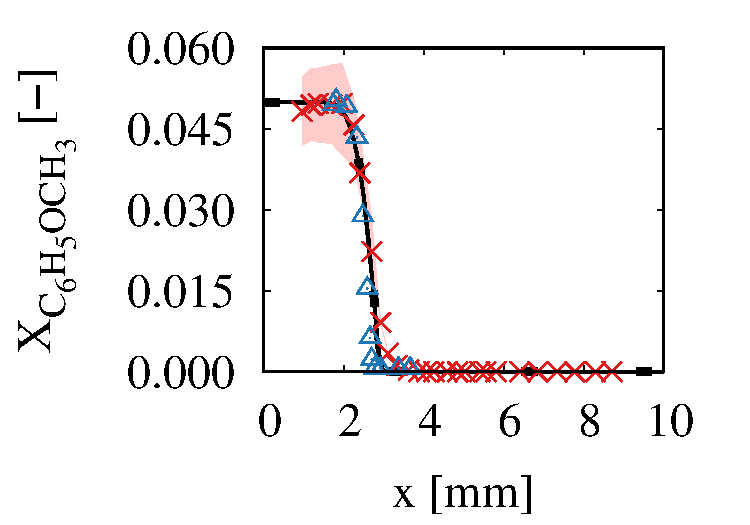
\includegraphics[width=0.32\textwidth]{\ThisPath Figures/B1b_Bio_Figure_6a.pdf}}
  \hfill
  \subfloat{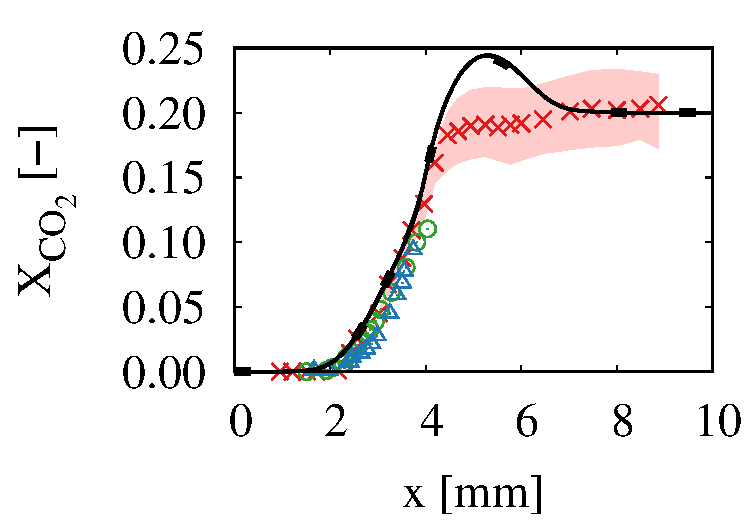
\includegraphics[width=0.32\textwidth]{\ThisPath Figures/B1b_Bio_Figure_6f.pdf}}
  \hfill
  \subfloat{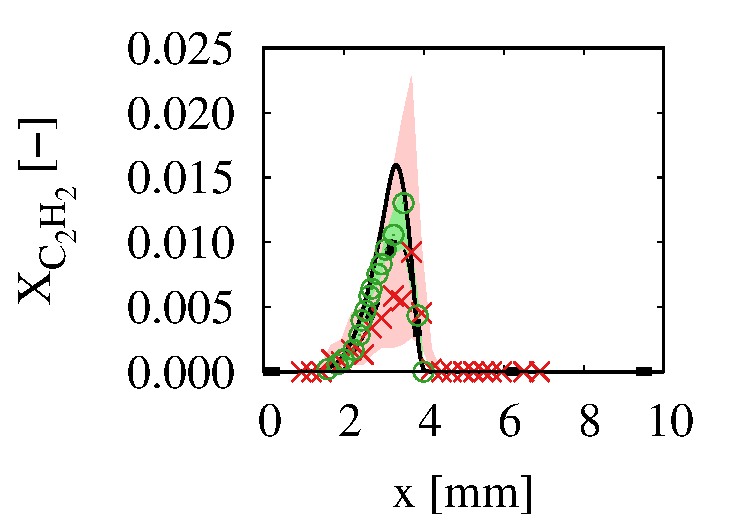
\includegraphics[width=0.32\textwidth]{\ThisPath Figures/B1b_Bio_Figure_8b.pdf}}
  \caption{Comparison of experimentally measured mole fractions in the \ce{CO2}O-Flame for anisole oxidation from Chen et al.~\cite{Chen2022} (ToF-MBMS: red crosses; GC-MS with a Rt-Q-Bond column: green circles; GC-MS with a DB-Petro column: blue triangles) with model predictions of the Skeletal-ITV-Bio (solid lines), the Merged-ITV-Anisole (dotted lines), and the LLNL-Anisole model~\cite{Wagnon2018} (dashed lines). Shaded areas with different colours indicate the measurement uncertainty of the respective techniques. x refers to the distance from the fuel inlet at 0 mm to the oxidizer inlet at 10 mm.}
  \label{fig:B1bAnisoleOxidationBioMechanismOXY}
\end{figure}
\\
The lignin combustion part of the Skeletal-ITV-Bio model is validated with the anisole oxidation in the \ce{CO2O} counterflow flame from Chen et al.~\cite{Chen2022}. Figure~\ref{fig:B1bAnisoleOxidationBioMechanismOXY} compares the experimental measurements with the model predictions of the Skeletal-ITV-Bio model, the Merged-ITV-Anisole, and the LLNL-Anisole model~\cite{Wagnon2018}. Anisole and \ce{CO2} mole fractions are well predicted with the Skeletal-ITV-Bio model, while the \ce{C2H2} formation is slightly over-predicted in comparison to the Merged-ITV-Anisole and the LLNL-Anisole model~\cite{Wagnon2018} as shown in Fig.~\ref{fig:B1bAnisoleOxidationBioMechanismOXY}.


\subsection{\ce{NOx} chemical kinetic sub-model}
\ce{NO_x} formation is validated for the Skeletal-ITV-\ce{NO_x} model for the volatile species released from the solid particle sub-model described in Cha.~\linkproject{A8} in a predefined range of validity against experimental data~\cite{Wu2022}.
\\
Figure~\ref{fig:B1bNOxWuValidation} compares the model predictions of the Skeletal-ITV-\ce{NO_x} with the model predictions of the Complete-ITV-\ce{NO_x} and the CRECK-\ce{NO_x} model~\cite{Shamooni2021} and with experimental measurements for fuel lean conditions from Wu et al.~\cite{ Wu2022}. The integrated \ce{C5H5N}-chemistry shows no discrepancies, while the \ce{NO} and \ce{NH3} model predictions from the ITV-based models are closer to the experimental measurements under these conditions than the CRECK-\ce{NO_x} model~\cite{Shamooni2021} predictions. Model predictions of the Skeletal-ITV-\ce{NO_x} and the Compact-ITV-\ce{NO_x} model show no discrepancies, indicating that the neglected pathways in the reduction step have only a minor error in the prediction accuracy of the target species.
\begin{figure}[h]
  \centering
  \subfloat{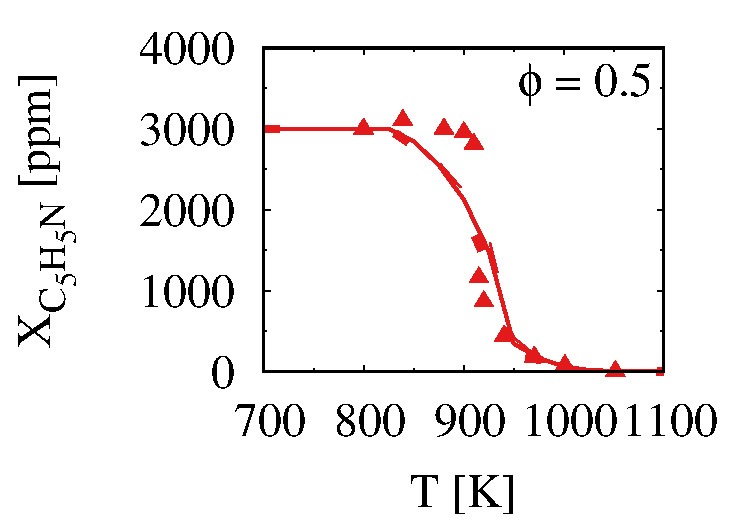
\includegraphics[width=0.32\textwidth]{\ThisPath Figures/B1b_NOx_Wu_Lean_C5H5N.pdf}}
  \hfill
  \subfloat{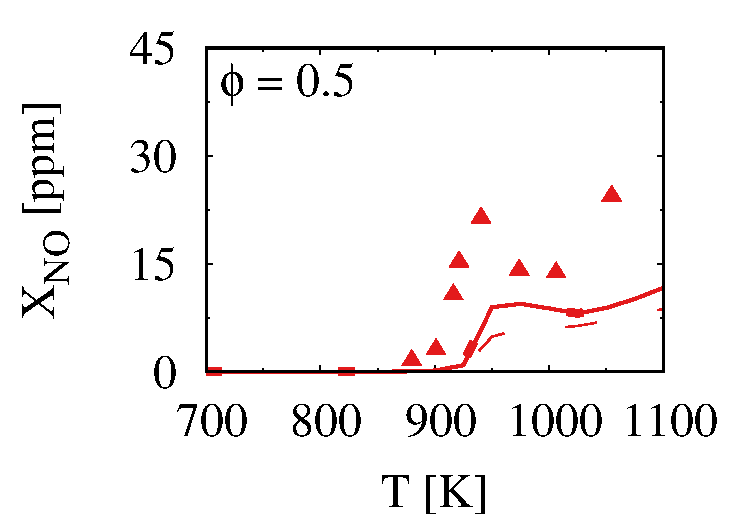
\includegraphics[width=0.32\textwidth]{\ThisPath Figures/B1b_NOx_Wu_Lean_NO.pdf}}
  \hfill
  \subfloat{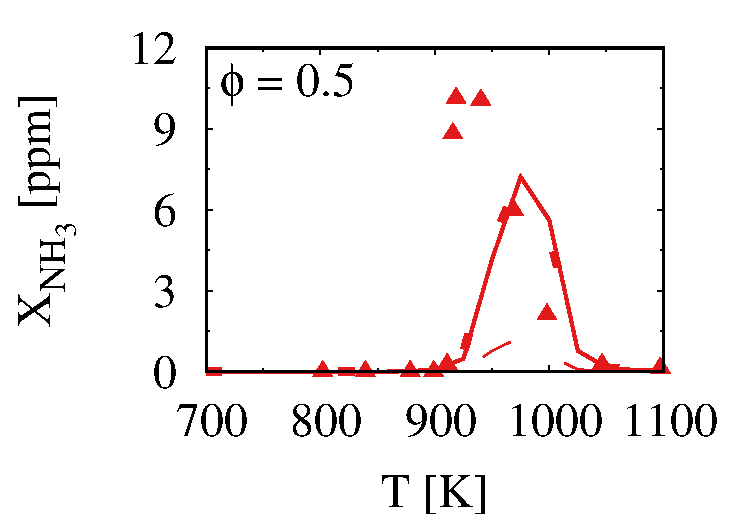
\includegraphics[width=0.32\textwidth]{\ThisPath Figures/B1b_NOx_Wu_Lean_NH3.pdf}}
  \caption{Comparison of experimental data from Wu et al.~\cite{Wu2022} in a jet-stirred reactor (symbols) with model predictions of the Skeletal ITV-\ce{NO_x} (solid lines), the Complete-ITV-\ce{NO_x} (dotted lines), and the CRECK-\ce{NO_x} model~\cite{Shamooni2021} (dashed lines).}
  \label{fig:B1bNOxWuValidation}
\end{figure}




%%%% DON'T CHANGE ANYTHING FROM HERE UNTIL NEXT MARKER!
\Acknowledgement

%\ThisPath 
\renewcommand{\bibname}{References}
\printbibliography[heading=subbibliography]

\end{refsection}
%%%% DONT CHANGE ANYTHING UNTIL HERE!
